\section{Waterfall Methodology}\label{sec:waterfall-methodology}
%https://en.wikipedia.org/wiki/Waterfall_model#History
The waterfall methodology was first introduced in the 1950's by Mr.
Benington but was only formalized in 1970 by  Winston W. Royce.
This methodology has been widely used in the industry, although it received
a lot of criticism few decades after.

This section will first present the key concepts of this methodology followed
by the detailed workflow.
After that, we'll point out the weaknesses of the model and present a
improved version of the model: the V-model.
Finally, we'll state the residual problems and limits of the improved model.

\subsection{Key concepts}\label{subsec:key-concepts}

The two main phases in software development are \textit{Analysis} and
\textit{Coding}.
Even projects with no clear methodology will at least go throw those two phases
that define and build the software.
However, these steps are only the emerged part of the iceberg.
Any software will require some specific design regarding its architecture, the
technologies it will use, its production environment and will also need time
to verify that the software actually works.


\begin{figure}
    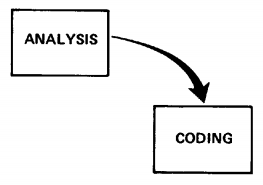
\includegraphics{waterfall/figure_1}
    \centering
\end{figure}


The problem stated by Royce is that these design and test steps were not very
well regarded, simply because they didn't directly add any business value.
Therefore, these steps were not very valuable from a client point of view and
were likely to be skipped. \\
Ignoring these steps often leads to horrific and costly overrun.
For example, fixing an architectural issue in a software might require a
complete new design and the developers will have to start all over again.
Also a lot of bugs will only be uncovered in production because of a lack
of testing effort, in terms of both strategy and execution.
New versions of the software will have to made to fix them, while hoping not
adding new problems.

Royce then proposed a model that adds extra steps to the development process,
in order to better design the software before implementing and releasing it.

We'll see more details later about the workflow itself.
The main improvement is that we now have more design steps, a dedicated step
for testing and the operations phase.
These steps that aren't directly related to the business value of the
software are now part of the nominal development process.

This emphasis on the design of the software makes this methodology very
\textit{document-oriented}.
This is one of the main traits of waterfall and there're a several types of
documents:
Software requirements, preliminary program design, interface design, final
program design, test plan and operations instructions.
These documents will help in several ways the project.

The formal aspect of written documents are nice during the design
specification by providing a tangible evidence of the understanding of a
requirement or the definition of a program interface.
A misunderstanding can easily be detected during a read over phase, by the
author, the analysts and the client.
This also prevent the project from forgetting a feature or any detail mentioned
during an informal meeting.

The documentation externalizes the knowledge from the analysts and clients
minds, which will benefit the whole project team.
Future maintainers of the application won't have to dig into the code base to
understand what it does, they will simply have to look at the structured
documentation to do so.

The test plan will be easier to made and execute, because we'll have a
comprehensive overview of the program and the expected behaviour.
While the developers are implementing the specification, the test team
(usually the analysts) can prepare all the test cases and data sets for the
testing phase at the end.

The operations phase will also take advantage of a well documented
application.
Installation or deployment processes will be clearly defined and even people
that never weren't there in the development phase will be able to start and
run the program.

\subsection{Workflow}\label{subsec:workflow}

\begin{figure}
    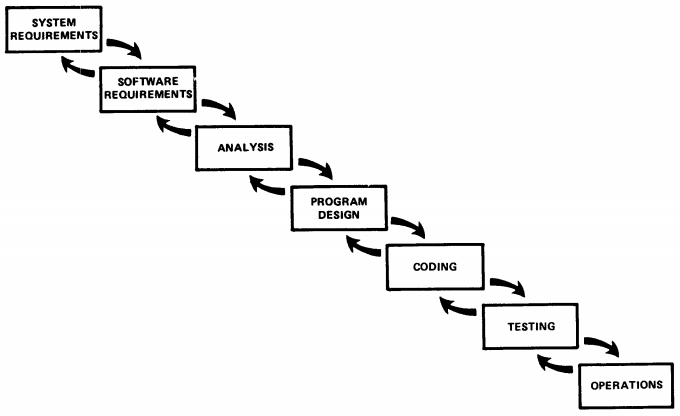
\includegraphics[scale=0.9]{waterfall/figure_2}
    \centering
\end{figure}

\subsection{Limits}\label{subsec:limits}

\subsection{V-Model}\label{subsec:v-model}